\chapter{Modelo econométrico}

%\noindent Este capítulo tiene el propósito de probar empíricamente las hipótesis planteadas previamente y está dividido en dos secciones.


\section{Análisis exploratorio de datos}

\noindent Con apoyo del área de \textit{analytics} del Sorteo Tec se obtuvo la base de datos con la cual se trabajaron los modelos econométricos para obtener la elasticidad ingreso y las relaciones funcionales buscadas. Además de esto, se utilizó información publicada por el Instituto Nacional de Estadística y Geografía (INEGI) relacionada a los niveles del PIB por Estado así como los datos de los censos poblacionales. \\

Se nos proporcionó información de tres sorteos los cuales, a continuación se presenta una breve descripción\footnote{Consulta realizada en \textit{www.sorteostec.org} el 6 de abril de 2020}: 

\begin{itemize}
    
    \item \textbf{AventuraT}: el boleto tiene un precio de \$140. Los premios de este sorteo van desde un viaje alrededor del mundo con valor de \$1,000,000 hasta certificados para compras de productos del Sorteo Tec por valor de \$140.
    
    \item \textbf{Educativo}: el boleto tiene un precio de \$300. Los premios de este sorteo van desde un certificado por una carrera completa en el Tecnológico de Monterrey, premio en efectivo por \$12,000,000 hasta un premio de \$300.
    
    \item \textbf{Mi Sueño}: el boleto tiene un precio de \$600. Los premios de este sorteo son en efectivo/cheque los cuales van desde un premio de \$28,000,000 hasta un premio de \$600.
    
    
\end{itemize}

La información que hay en la base de datos proporcionada por el Sorteo Tec contiene datos de los tres sorteos mencionados anteriormente. Para cada sorteo se tiene el número de boletos vendidos por oficina en cada Estado y la fecha en la cual se celebró cada sorteo. \\

%11/10/2020

A continuación se presentan los Estados en los cuales se tiene registro de ventas de boletos del Sorteo Tec. Es importante mencionar que, no en todos los Estados del país existe un campus Tec de Monterrey pero, sí existen oficinas de representación en las cuales se pueden comprar boletos. La base de datos cuenta con información de 30 Estados y una oficina virtual, a los cuales se les asignó un ID y una variable indicadora si en dicho Estado hay un campus Tec de Monterrey. \\

\begin{table}[H]
\caption{Estados en donde se venden boletos del Sorteo Tec}
\label{edos}
\centering
\scalebox{0.8}{
\begin{tabular}{rrll}
  \hline
 ID & Estado & Campus \\ 
  \hline
  1 & Aguascalientes & Si \\ 
  2 & Baja California & No \\ 
  3 & Baja California Sur & No \\ 
  4 & Coahuila de Zaragoza & Si \\ 
  5 & Colima & Si \\ 
  6 & Chiapas & Si \\ 
  7 & Chihuahua & Si \\ 
  8 & Distrito Federal & Si \\ 
  9 & Durango & No \\ 
  10 & Guanajuato & Si \\ 
  11 & Guerrero & No \\ 
  12 & Hidalgo & Si \\ 
  13 & Jalisco & Si \\ 
  14 & Estado de Mexico & Si \\ 
  15 & Michoacan de Ocampo & Si \\ 
  16 & Morelos & Si \\ 
  17 & Nayarit & No \\ 
  18 & Nuevo Leon & Si \\ 
  19 & Oaxaca & No \\ 
  20 & Puebla & Si \\ 
  21 & Queretaro & Si \\ 
  22 & Quintana Roo & No \\ 
  23 & San Luis Potosi & Si \\ 
  24 & Sinaloa & Si \\ 
  25 & Sonora & Si \\ 
  26 & Tabasco & No \\ 
  27 & Tamaulipas & Si \\ 
  28 & Veracruz de Ignacio de la Llave & Si \\ 
  29 & Yucatan & No \\ 
  30 & Zacatecas & Si \\ 
  31 & Oficina Virtual & No \\ 
   \hline
\end{tabular}
}
\end{table}


Se transformó esta información para poder llegar al número de boletos vendidos por Estado. A continuación, a manera de ejemplo, se presentan las primeras seis observaciones de la tabla que resulta del manejo de datos para el sorteo AventuraT:

\begin{table}[H]
\caption{Datos para el sorteo AventuraT}
\label{aven}
\scalebox{0.8}{
\begin{tabular}{ccccccc}
\hline
\multicolumn{1}{l}{Estado}              & \multicolumn{1}{1}{ID} & \multicolumn{1}{l}{Fecha} & \multicolumn{1}{l}{\# Boletos} & \multicolumn{1}{l}{PIB \textit{per capita} } & \multicolumn{1}{l}{PIB*} & \multicolumn{1}{1}{Campus} \\ \hline
Aguascalientes                          & 1  & 4/dic/2015                & 553                            & 150,985.72                 & 198,175.39               & Sí     \\
Baja California                         & 2  & 4/dic/2015                & 1498                           & 152,585.45                 & 505,937.66               & No     \\
Baja California Sur                     & 3  & 4/dic/2015                & 953                            & 182,712.47                 & 130,096.58               & No     \\
Coahuila de Zaragoza                    & 4  & 4/dic/2015                & 4650                           & 194,201.89                 & 573,850.07               & Sí     \\
Colima                                  & 5  & 4/dic/2015                & 1725                           & 134,073                    & 95,357.74                & Sí     \\
Chiapas                                 & 6  & 4/dic/2015                & 389                            & 55,666                     & 290,463.61               & Sí     \\ \hline
\multicolumn{1}{l}{*Cifras en millones de pesos} &    &                           &                                &                            &                          &        \\ 
\end{tabular}
}
\centering
\source{Fuente: Elaboración propia con datos del Sorteo Tec}

\end{table} \\

Con la información obtenida para cada sorteo se realizaron diferentes visualizaciones para obtener mayor información acerca de los datos. En primer lugar se presenta un diagrama de cajas y brazos, diferenciando en grupos si existe un campus Tec de Monterrey en el Estado, en donde se observa que para los 3 sorteos los Estados que más boletos vendieron entre 2015 y 2019 son Nuevo León, Tamaulipas, Jalisco y la Oficina Virtual. En estos primeros 3 estados existe un campus Tec de Monterrey, lo cual puede darnos una idea si el hecho de que exista un campus en el Estado tenga un efecto sobre el número de boletos vendidos.

\begin{figure}[H]
    \caption{Boletos vendidos por Estado}
    \label{fig:boxplot}
    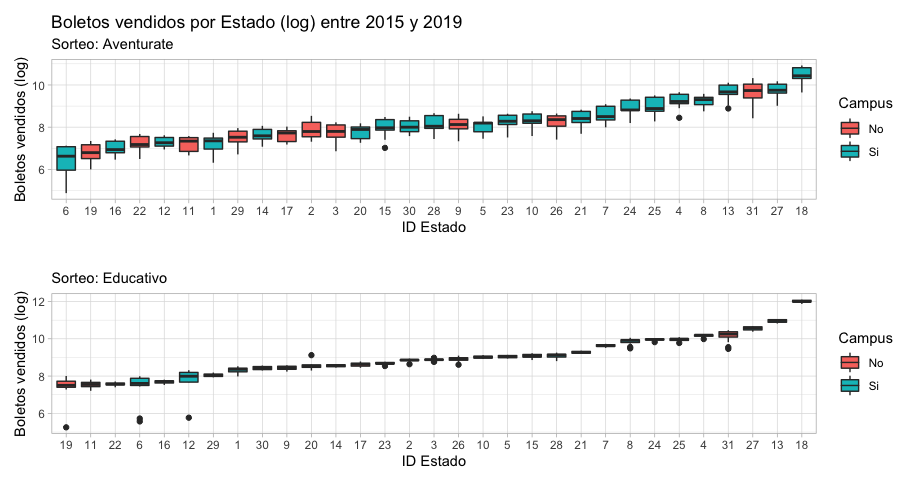
\includegraphics[scale = 0.43]{Imagenes/boxplot1.png}
    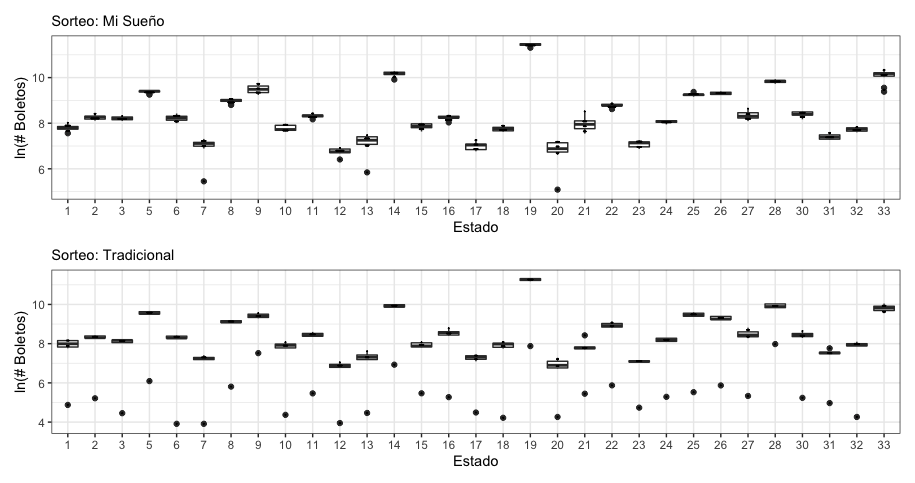
\includegraphics[scale = 0.43]{Imagenes/boxplot2.png}
    \centering
    \imagesource{Elaboración propia}
\end{figure}


En relación a lo anterior, se presenta la matriz de correlaciones entre las variables: 

\begin{itemize}
    \item \textit{campus}: variable indicadora si existe un campus en el Estado o no.
    \item \textit{pib\_pc}: PIB \textit{per capita} por Estado en escala logarítimica. \\
    \item \textit{n\_boletos}: número de boletos vendidos por Estado en escala logarítmica.
\end{itemize} \\

\begin{figure}[H]
    \caption{Matriz de Correlación por Sorteo}
    \label{fig:corplot}
    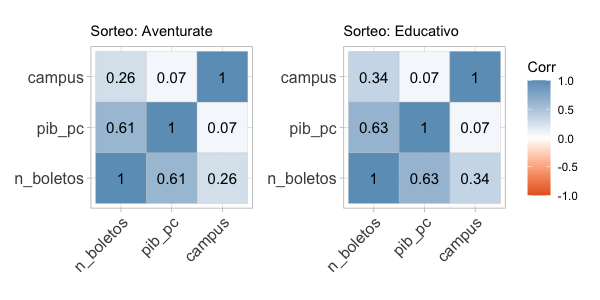
\includegraphics[scale = 0.4]{Imagenes/cp1.png} \\
    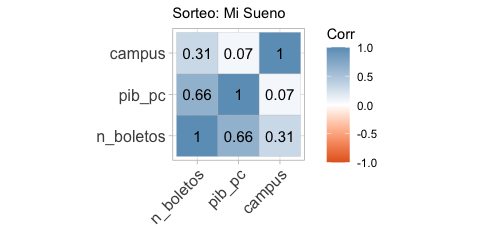
\includegraphics[scale = 0.5]{Imagenes/cp2.png} \\
    \centering
    \imagesource{Elaboración propia}
\end{figure} 

Se observa que para los 3 sorteos hay una correlación positiva alta entre las variables \textit{n\_boletos} y \textit{pib\_pc}, mientras que la correlación entre las variables \textit{campus} y \textit{n\_boletos} si bien es positiva no tiene un nivel alto a excepción en los sorteos Educativo y Mi Sueño. \\

Por otro lado, se analizó la variable de boletos vendidos por Estado. Primero observamos que el sorteo Educativo es el que más boletos ha vendido entre 2015 y 2019, esto se podría explicar debido a que cierto grupo de alumnos de la institución tienen que vender cierta cantidad de boletos ligado a alguna ayuda financiera que la Institución les esté otorgando.
    
\begin{figure}[H]
    \caption{Boletos vendidos por sorteo}
    \label{fig:bolvendidos}
    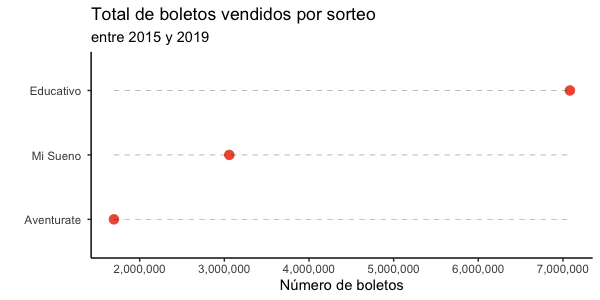
\includegraphics[scale = 0.5]{Imagenes/n_boletos.png} \\
    \centering
    \imagesource{Elaboración propia}
\end{figure} 

Ahora bien, observamos esta misma información pero agrupada de diferente manera. Agrupamos el número de boletos vendidos por Estado y observamos que entre 2015 y 2019 el Estado que vendió más boletos fue Nuevo León. Esto se podría explicar debido a que la Institución nace en este Estado y la presencia del número de docentes, alumnos y personal es significativamente mayor en comparación a otros Estados. Si bien, como se observó en la figura 3.2 la correlación entre que haya un campus en el Estado no tiene una correlación positiva elevada, se observa en las siguientes gráficas que para todos los sorteos los Estados que más boletos venden son los que tienen un campus Tec de Monterrey.

\begin{figure}[H]
    \caption{Boletos vendidos por Estado}
    \label{fig:bolvendidos}
    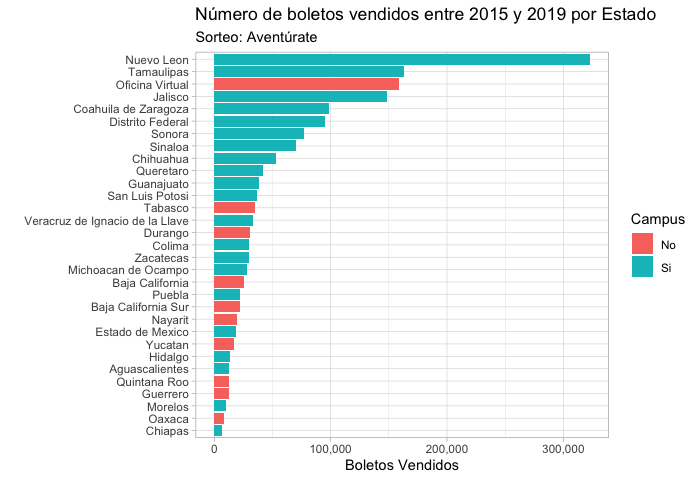
\includegraphics[scale = 0.5]{Imagenes/boletos_av.png} \\
    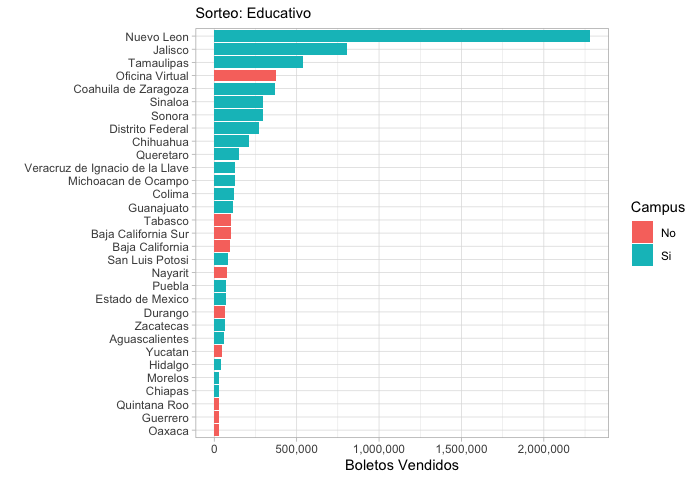
\includegraphics[scale = 0.5]{Imagenes/boletos_ed.png} \\
    \centering
%    \imagesource{Elaboración propia}
\end{figure} \\

\begin{figure}[H]
%    \caption{Boletos vendidos por Estado}
    \label{fig:bolvendidos2}
    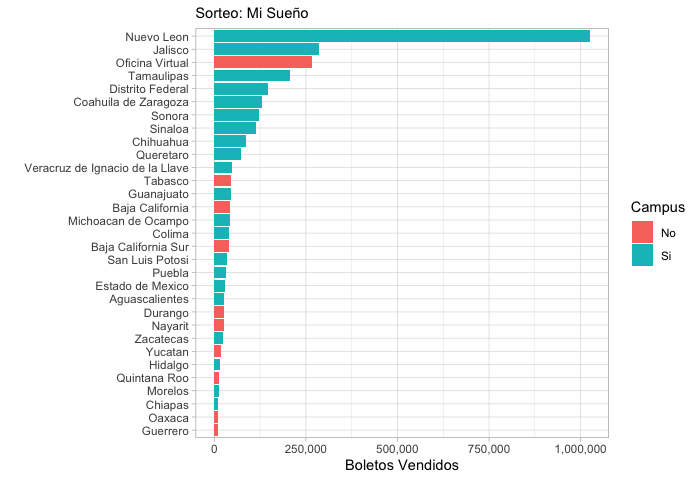
\includegraphics[scale = 0.5]{Imagenes/boletos_sue.png} \\
    \centering
     \imagesource{Elaboración propia}
\end{figure} 

De igual forma, se observaron los 15 Estados que vendieron más boletos entre 2015 y 2019 para analizar como se comportaron las ventas en cada fecha de sorteo. Para el sorteo Aventúrate se observa una tendencia creciente en el número de boletos vendidos  y apartir de 2018 se ve una clara disminución para los 15 Estados. Para los otros 2 sorteos no se observa una tendencia clara. Es importante mencionar que, en la selección de estas 15 entidades se observan Estados que no cuentan con un campus Tec de Monterrey en él.

\begin{figure}[H]
    \caption{Estados que más boletos vendieron}
    \label{fig:bolvendidos_top}
    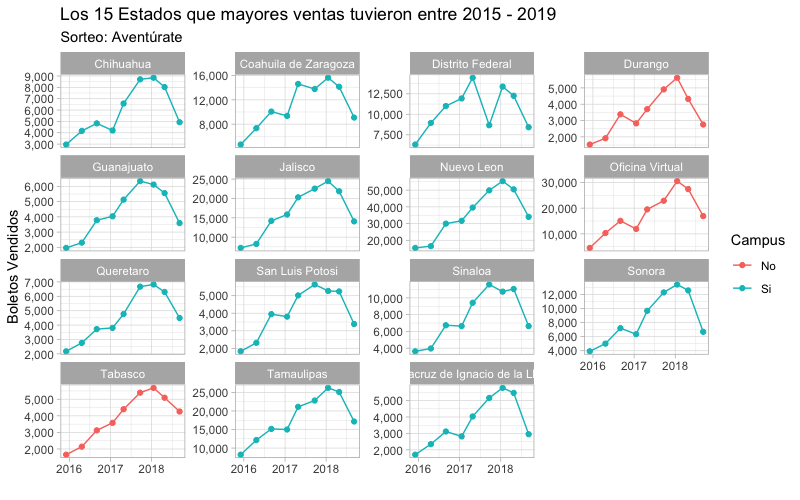
\includegraphics[scale = 0.5]{Imagenes/aven_15edos.png} \\
    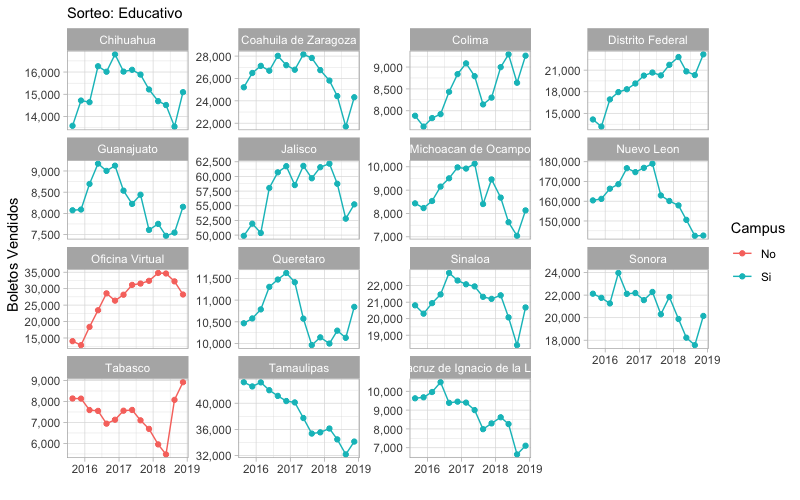
\includegraphics[scale = 0.5]{Imagenes/educ_15edos.png} \\
    \centering
%    \imagesource{Elaboración propia}
\end{figure} \\

\begin{figure}[H]
%    \caption{Boletos vendidos por Estado}
    \label{fig:bolvendidos_top2}
    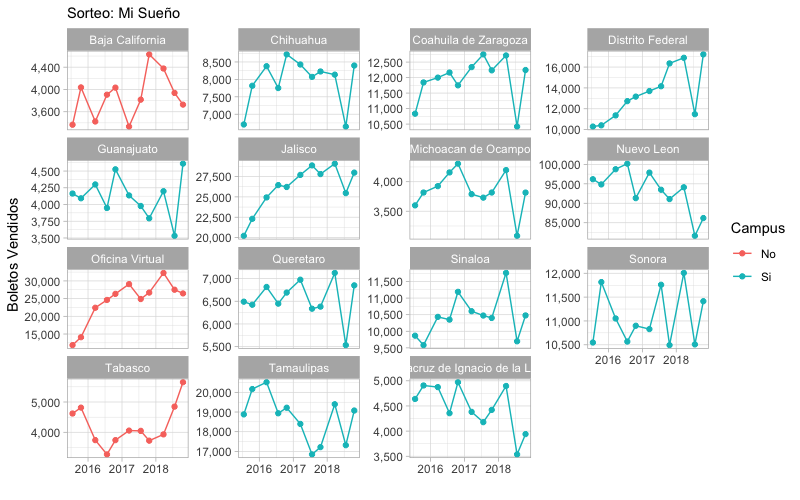
\includegraphics[scale = 0.5]{Imagenes/sue_15edos.png} \\
   % 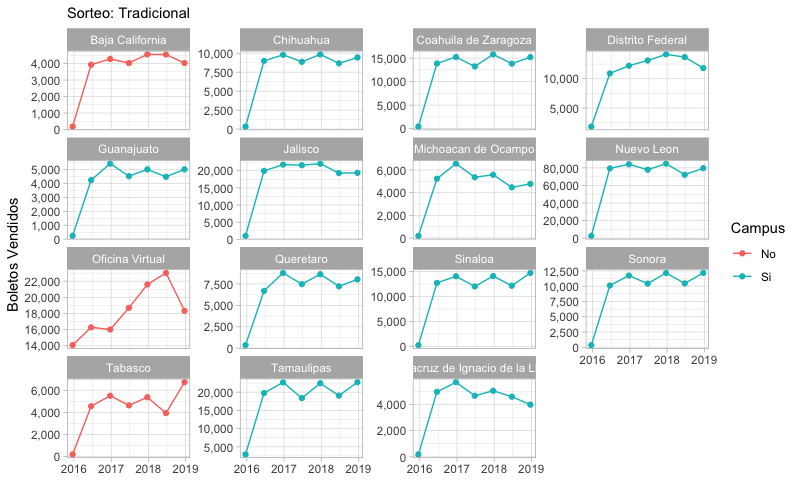
\includegraphics[scale = 0.5]{Imagenes/trad_15edos.png} \\
    \centering
    \imagesource{Elaboración propia}
\end{figure} 

Por otro lado, se buscó encontrar la relación existente entre el número de boletos vendidos y el PIB \textit{per capita} (aplicando logaritmos a las dos variables para cada sorteo). Esto con la intención de analizar más a fondo lo observado en la figura 3.2.

\begin{figure}[H]
    \caption{Boletos vs PIB \textit{per capita} (log - log)}
    \label{fig:scat}
    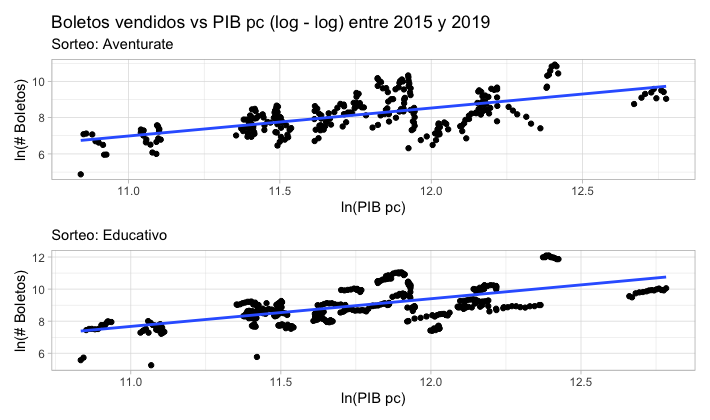
\includegraphics[scale = 0.35]{Imagenes/sc1.png}
    \centering
    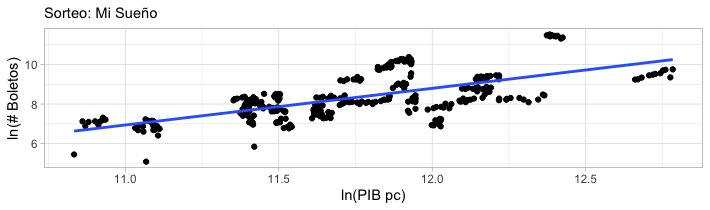
\includegraphics[scale = 0.35]{Imagenes/sc2.png} \\
    \centering
    \imagesource{Elaboración propia}
\end{figure}

De las gráficas anteriores, se observa una clara relación positiva entre el logaritmo natural del número de boletos vendidos y el logaritmo natural del PIB \textit{per capita}. Esto resulta relevante pues, como se mencionó en el capítulo anterior, la elasticidad ingreso nos mide la sensibilidad en la cantidad demandada de un bien cuando cambia el ingreso. Observar esta relación positiva nos empieza a dar señales de cómo será esta elasticidad. \\

%Por otro lado, observamos que para los cuatro sorteos el Estado en donde se registraron el mayor número de boletos vendidos fue Nuevo León. Un aspecto relevante es que entre los años 2015 y 2019 Nuevo León fue el tercer Estado con un PIB promedio más alto como se ve en la siguiente gráfica.

%\begin{figure}[H]
%    \centering
%    \caption{PIB por Estado}
%    \label{fig:box-pib}
%    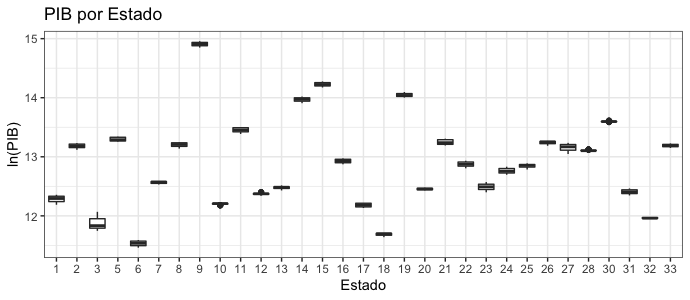
\includegraphics[scale = 0.5]{Imagenes/boxplot_pib.png}
%    \imagesource{Elaboración propia}
%\end{figure}





\newpage

\section{Modelo}

\noindent Para la comprobación de la hipótesis propuesta para esta tesis, se corrieron diferentes modelos de regresión tanto log-log como múltiple. \\

Los modelos econométricos que se utilizarán en este trabajo son los siguientes:

\begin{equation}
    ln(y) = \beta_0 + \beta_1 ln(x) + \epsilon
\end{equation}

\begin{equation}
    y = \alpha_0 + \alpha_1 x + \alpha_2 x^2 + \epsilon
\end{equation}
 
Donde $y$ es el número de boletos vendidos, $x$ es el PIB \textit{per capita} y $\epsilon \sim N(0,\sigma^2)$ para ambos modelos. Estos modelos nos servirán para encontrar con la ecuación (3.1) la elasticidad ingreso y con la ecuación (3.2) la concavidad de la función. \\

El modelo (3.1) se origina de la siguiente manera. Consideremos el siguiente modelo que se conoce como \textit{regresión exponencial}:

\begin{equation}
    Y_i = \theta_0 X_{i}^{\beta_1} e^{u_i}
\end{equation}

El cual puede ser expresado de la siguiente forma:

\begin{equation}
    ln (Y_i) = \beta_0 + \beta_1 ln (X_i) + u_i
\end{equation}

Donde $\beta_0 = ln (\theta_0)$. A la ecuación (3.4) se le conoce como \textbf{modelo log-log}, este modelo resulta ser lineal en los parámetros $\beta_0$ y $\beta_1$, lineal en los logaritmos de las variables Y y X. De aquí se sigue que, si los supuestos de una regresión lineal clásica se cumplen, los parámetros pueden ser estimados mediante mínimos cuadrados ordinarios sustituyendo $Y_i^* = ln (Y_i)$ y $X_i^* = ln(X_i)$ llegando a la siguiente ecuación:

\begin{equation}
    Y_i^* = \beta_0 + \beta_1X_i^* + u_i
\end{equation}

Se propone el modelo log-log debido a que el coeficiente $\beta_1$ mide la elasticidad de Y respecto a X. Es importante mencionar que, el modelo asume que la elasticidad es constante a través de toda la curva, en otras palabras esto significa que el cambio en $ln(Y)$ debido al cambio en $ln(X)$ permanece constante sin importar a que nivel de $ln(X)$ se esté midiendo la elasticidad. \\

Traduciéndolo a nuestro contexto, si tomamos el modelo (3.1) con nuestras variables tenemos que:

\begin{equation}
    \beta_1 = \frac{\Delta \: \% \:boletos \: vendidos}{\Delta \: \% \: PIB \: pc} \equiv \varepsilon_{I,x}
\end{equation} \\


Así, obtenemos la elasticidad ingreso de los boletos del Sorteo Tec la cual es parte central de nuestra investigación. \\

Ahora, el modelo (3.2) nos explicará si existe una forma funcional cóncava o convexa, esto se obtiene del coeficiente $\alpha_2 = \frac{\partial^2 y}{\partial x^2}$ del cual nos interesa el signo. Traduciéndolo a nuestro contexto con nuestras variables, tenemos que:

\begin{equation}
    \alpha_2 = \frac{\partial^2 \:boletos \: vendidos}{\partial PIB \: pc^2}
\end{equation}

Si $\alpha_2 < 0$ tenemos una función cóncava y si $\alpha_2 > 0$ tenemos una función convexa. Bajo nuestra hipótesis, esperaríamos que la función fuera cóncava lo cual nos daría una idea de que el individuo es averso al riesgo como se explicó en el capítulo \textbf{2.1}. \\

Estos modelos se utilizarán para los 3 sorteos y así analizar cada uno por separado. A continuación, en el \textbf{cuadro 3.3} se presenta el ajuste que se realizó para el modelo (3.1) y en el \textbf{cuadro 3.4} se presenta el ajuste que se realizó para el modelo (3.2). El ajuste se realizó con el método de mínimos cuadrados ordinarios y se utilizó el software estadístico R. La validación de los modelos se encuentra en los apéndices A y B. \\

%Regresiones para los 4 sorteos: modelo ln(y) ~ ln(x)

\begin{table}[H] 
\centering 
  \caption{Ajuste Modelo (3.1)} 
  \label{lm_loglog} 
\scalebox{0.65}{
\begin{tabular}{@{\extracolsep{5pt}}lccc} 
\\[-1.8ex]\hline 
\hline \\[-1.8ex] 
 & \multicolumn{3}{c}{\textit{Dependent variable:}} \\ 
\cline{2-4} 
\\[-1.8ex] & \multicolumn{3}{c}{log(Venta Estado)} \\ 
\\[-1.8ex] & (AventuraT) & (Educativo) & (Mi Sueño)\\ 
\hline \\[-1.8ex] 
 log(PIB \textit{per capita}) & 1.542$^{***}$ & 1.726$^{***}$ & 1.854$^{***}$ \\ 
  & (0.120) & (0.103) & (0.113) \\ 
  & & & \\ 
 Constant & $-$9.979$^{***}$ & $-$11.317$^{***}$ & $-$13.448$^{***}$ \\ 
  & (1.417) & (1.211) & (1.335) \\ 
  & & & \\ 
\hline \\[-1.8ex] 
R$^{2}$ & 0.372 & 0.395 & 0.441 \\ 
Adjusted R$^{2}$ & 0.370 & 0.393 & 0.440 \\ 
Residual Std. Error & 0.809 (df = 277) & 0.861 (df = 431) & 0.835 (df = 338) \\ 
F Statistic & 163.937$^{***}$ (df = 1; 277) & 281.194$^{***}$ (df = 1; 431) & 266.968$^{***}$ (df = 1; 338) \\ 
\hline 
\hline \\[-1.8ex] 
\textit{Note:}  & \multicolumn{3}{r}{$^{*}$p$<$0.1; $^{**}$p$<$0.05; $^{***}$p$<$0.01} \\ 
\end{tabular} 
}
\end{table} 

%Regresiones para los 4 sorteos: modelo y ~ x + x^2

\begin{table}[H] 
\centering 
  \caption{Ajuste Modelo (3.2)} 
  \label{cuadratic_model} 
\scalebox{0.65}{
\begin{tabular}{@{\extracolsep{5pt}}lccc} 
\\[-1.8ex]\hline 
\hline \\[-1.8ex] 
 & \multicolumn{3}{c}{\textit{Dependent variable:}} \\ 
\cline{2-4} 
\\[-1.8ex] & \multicolumn{3}{c}{Venta Estado} \\ 
\\[-1.8ex] & (AventuraT) & (Educativo) & (Mi Sueño)\\ 
\hline \\[-1.8ex] 
 PIB \textit{per capita} & 0.120$^{***}$ & 0.418$^{***}$ & 0.221$^{***}$ \\ 
  & (0.028) & (0.084) & (0.054) \\ 
  & & & \\ 
  
 (PIB \textit{per capita})^2 & $-$1.613e-07$^{**}$ & $-$5.713e-07$^{**}$ & $-$2.588e-07$^{*}$  \\ 
  & (7.606e-08) & (2.291e-07) & (1.471e-07) \\ 
  & & & \\ 
 Constant & $-$6,909.530$^{***}$ & $-$28,626.400$^{***}$ & $-$15,784.160$^{***}$ \\ 
  & (2,285.693) & (6,858.514) & (4,410.503) \\ 
  & & & \\ 
\hline \\[-1.8ex] 
R$^{2}$ & 0.222 & 0.194 & 0.208 \\ 
Adjusted R$^{2}$ & 0.216 & 0.191 & 0.204 \\ 
Residual Std. Error & 7,136.310 (df = 276) & 26,589.100 (df = 430) & 15,011.720 (df = 337) \\ 
F Statistic & 39.377$^{***}$ (df = 2; 276) & 51.861$^{***}$ (df = 2; 430) & 44.358$^{***}$ (df = 2; 337) \\ 
\hline 
\hline \\[-1.8ex] 
\textit{Note:}  & \multicolumn{3}{r}{$^{*}$p$<$0.1; $^{**}$p$<$0.05; $^{***}$p$<$0.01} \\ 
\end{tabular}  
}
\end{table} \\

Como comentario adicional, se ajustaron dos modelos más, al modelo 3.1 y al modelo 3.2 se les agregó una variable indicadora que corresponde a la existencia de un campus Tec en el Estado, esto con la intención de ver el efecto fijo que podría presentar tanto en la estimación de la elasticidad como en la concavidad de la función. Los resultados de dicho ajuste no presentaron diferencias significativas a los presentados en las tablas anteriores (se preservaron las magnitudes y los signos).


% Para escribir ecuaciones

%\begin{table}[H]
%\centering
%\caption{Resultados del modelo econométrico}
%\label{REG}
%\begin{tabular}{|ccccc|}
%  \hline
% & Estimador & Desv. est. & Valor $t$ & Pr($>|t|$) \\ 
%  \hline
%  $\alpha$ & x & x & x & x \\ 
%  CI & x & x & x & x \\ 
%  IS & x & x & x & x \\ 
%  IR & x & x & x & x \\ 
%  PT & x & x & x & x \\ 
%   \hline
%\multicolumn{5}{|c|}{Error est. de res. = x con x gr. de libertad}
%    \\
%    \multicolumn{5}{|c|}{$R^2$ = x y $\bar{R}^2$ = x}
% \\
% \multicolumn{5}{|c|}{Estadístico $F$ = x, con un valor $p$ = x }
%      \\
%\hline
%\end{tabular} \\

%\end{table}
